\documentclass[a4]{scrartcl}

% \usepackage[ngerman]{babel}
\usepackage[utf8]{inputenc}
\usepackage{mathtools}
\usepackage{amsmath}
\usepackage{amssymb}
\usepackage{geometry}
\usepackage{scrlayer-scrpage}
\usepackage{float}
\pagestyle{scrheadings}
\usepackage{xcolor}
\clearscrheadfoot

\usepackage[backend=biber, maxbibnames=99]{biblatex}
\addbibresource{references.bib}

\setlength{\parindent}{0cm}


\geometry{
  paper=a4paper, % Change to letterpaper for US letter
  top=2cm, % Top margin
  bottom=1.5cm, % Bottom margin
  left=2cm, % Left margin
  right=3cm, % Right margin
}

\usepackage[framemethod=TikZ]{mdframed}

% Style %
\mdfdefinestyle{enviStyle}{
   innertopmargin = 10pt,
  linewidth      = 1pt,
  frametitlerule = true,
  roundcorner    = 2pt%
}





\newenvironment{CountingDefinition}[2][]{%
   \ifstrempty{#1}%
   {\mdfsetup{%
      frametitle={{\strut Problem~}}}
   }%
   {\mdfsetup{%
      frametitle={{\strut Problem:~#1}}}%
   }%
   \mdfsetup{
      nobreak                   = true,
     linecolor                 = gray,
    frametitlebackgroundcolor = gray!50,
    style                     = enviStyle
   }
   \begin{mdframed}[]\relax%
   \label{#2}}{\end{mdframed}}




\ohead{\\
Pina Kolling\\
piko0011}

\begin{document}


%-------------------------------------------------------------------




\section*{Summary: Lecture 3}

Summary for the chapter \textit{7.5} until page 150. \cite{CC, book}

%-------------------------------------------------------------------



\subsection*{Background knowledge}

The P vs. NP problem is an unsolved problem in complexity theory.
Mathematical problems which are solved by a computer are classified as P or NP problems: All problems that can be solved efficiently by a computer belong to the class P. In the case of NP problems it is unknown whether they can be solved efficiently or not. In this context, efficient means that the required computing time of a solution algorithm grows at most polynomially (e.g. quadratically) with increasing complexity. The only thing that is currently clear is that a correct solution to an NP problem can be checked for correctness in polynomial time. 

Developing an algorithm for an NP problem is usually very difficult. Computer scientists and mathematicians do not only try to work out effective algorithms, they also try to determine whether P = NP. In other words, they are trying to find out whether P and NP are really different problem classes or whether it is possible to solve NP problems in polynomial time as well. Scientists all over the world are trying to prove that P != NP. 

The reason why experts wish NP problems to remain almost unsolvable is called cryptography. Unlike many other fields, complexity in cryptography is not only desirable, but necessary. It is important to know that most encryption methods used today are based solely on the fact that the effort to \textit{guess} the key is too high. The problem of \textit{guessing} is therefore an NP problem. Not only theoretically, but also practically, the proof of the solvability of NP problems means the end of all currently used encryption methods.

But there is still hope for cryptography. The NP problem has often been supposedly solved. Both P = NP and P != NP have been attempted to be proven many times. It turned out that every single solution and every single proof attempt so far turned out to be wrong or incomprehensible. \cite{DD, book, GTI}



%-------------------------------------------------------------------



\subsection*{Basic relations between complexity classes}


The hierarchy theorem shows how deterministic classes of the same kind (time or space) relate to each other.
Here are the relationships between classes of a different kind exmined: P and NP.

If $f(n)$ is a proper complexity function:
\begin{align}
& \text{SPACE}(f(n)) \subseteq \text{NSPACE}(f(n)) \text{ and TIME}(f(n)) \subseteq \text{NTIME}(f(n)) \\
& \text{NTIME}(f(n)) \subseteq \text{SPACE}(f(n)) \\
& \text{NSPACE}(f(n)) \subseteq \text{TIME}(k^{\log n + f(n)}) 
\end{align}

\textbf{Proof for $(1)$:} \\
Any deterministic Turing Machine is also a non-deterministic Turing Machine, which leads to $\text{SPACE}(f(n)) \subseteq \text{NSPACE}(f(n)) \text{ and TIME}(f(n)) \subseteq \text{NTIME}(f(n))$.

\ \\
\textbf{Proof for $(2)$:} \\
To prove $(2)$, a language $L \in $ NTIME$(f(n))$ is considered. It exists a precis non-deterministic Turing Machine $M$ that decides $L$ in time $f(n)$ and for the prove a deterministic Turing Machine $M'$ has to be designed that decides $L$ in space $f(n)$.
Memory space can be reused, time cannot.
There are $d$ choices in every step: $1,...,d$. For each choice the non-determinstic Turing Machine is simulated and the previous simulations can be deleted to reuse space. Only the currently simulated and the next simulation need to be saved and tracked.


\ \\
\textbf{Proof for $(3)$:} \\
This proof involves a method for space-bounded Turing Machines, which is called \textbf{reachability method}.
For this, a multistring non-deterministic Turing Machine $M$ with input and output is given, which decides a lanugage $L$ within space $f(n)$.
Then things happen and graphs/graph edges are constructed, $M$ empties the tape and puts all the heads to the start and there is only a single node that is accepting.


\ \\ \\
Combining the previous knowledge, it can be concluded:
\begin{center}
L $\subseteq$ NL $\subseteq$ P $\subseteq$ NP $\subseteq$ PSPACE
\end{center}
and
\begin{center}
L $\subset$ PSPACE
\end{center}
This means, that at least on of the inclusions has to be proper.

\ \\
\color{violet} Questions: What happens in the reachability method proof?!
\color{black}


%-------------------------------------------------------------------


\begin{CountingDefinition}[GRAPH REACHABILITY]{def:validLabelPlacement}
Given a graph $G$ and two nodes $n_1, n_2 \in V$, is there  path from $n_1$ to $n_2$?

(A graph $G=(V, E)$ is a finite set $V$ of nodes and a set $E$ of edges (node pairs). )
\end{CountingDefinition}


%-------------------------------------------------------------------
\subsection*{Savitch's theorem}
\begin{align*}
\text{REACHABILITY} \in \text{SPACE}(\log^2 n)
\end{align*}

\textbf{Proof:} \\
PATH$(startnode, endnode, m)$ checks if there is a path from startnode to endnode with the length of at most $2^m$. 

The parameters of the function can be split up (like divide and conquer):
\begin{align*}
\text{PATH}(i,j,m) \Leftrightarrow \exists k : \text{PATH}(i,k,m-1) \text{ and PATH}(k,j,m-1) 
\end{align*}
Some internal node $k$ is choosen and it is checked recursively if there is a path from $startnode$ to $k$ and from $endnode$ to $n$. This is then recursively done with the new midpoint. \\


There can be $\log n$ many segments to work on -- the recursion depth and the record size both are at most $\log n$. This leads to a recursion stack of $O(\log^2 n)$.


The complexity function is at least $\log n$.




\begin{figure}[H]
\begin{center}
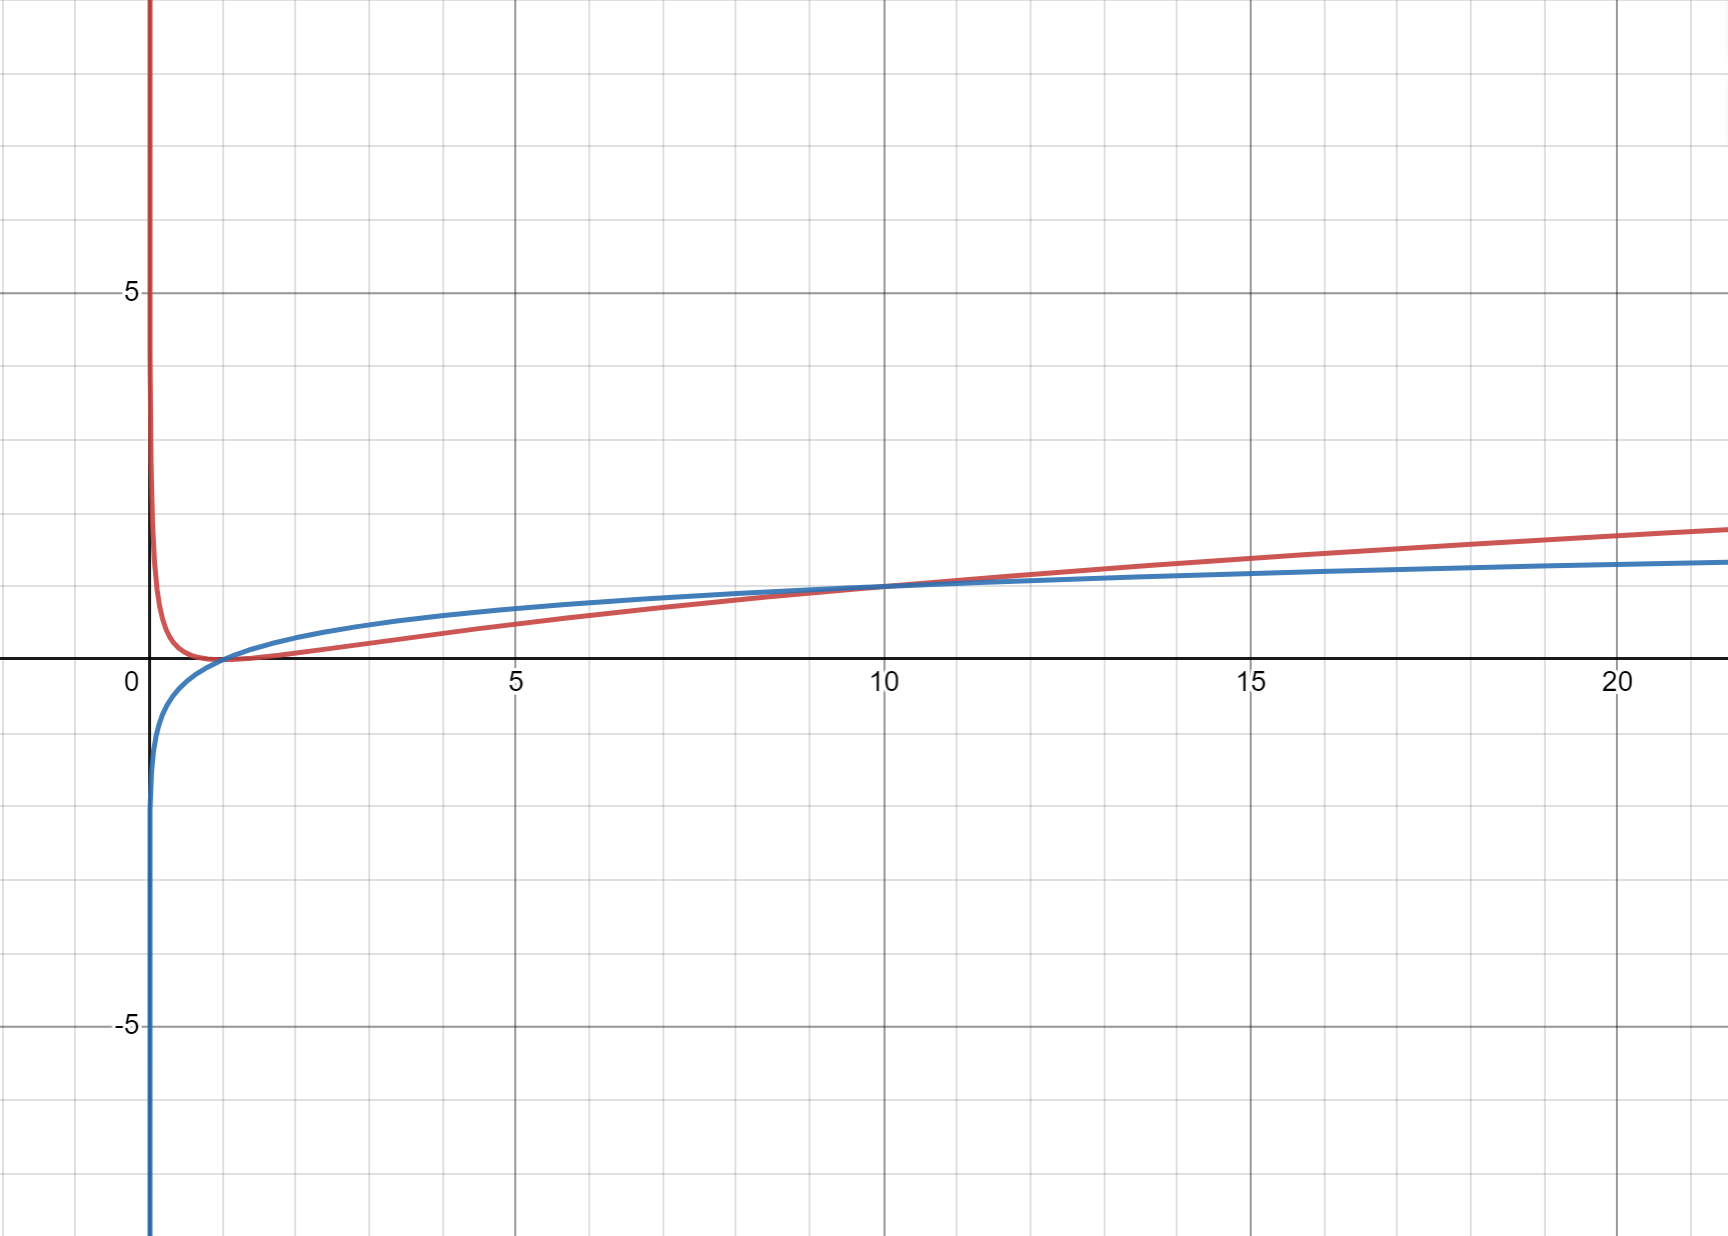
\includegraphics[scale=0.3]{images/logplot.png}
\caption{Red graph $f(n) = \log ^2 n$ and blue graph $g(n)= \log n$}
\end{center}
\end{figure}



\color{violet} Questions: Why does the meaning of $n$ change?
\color{black}



%-------------------------------------------------------------------
\subsection*{Analysis}
imagine the graph \\
graph can be too large to construct \\




\color{red} TODO
\color{black}

\color{violet} Questions:
\color{black}














%-------------------------------------------------------------------

\newpage

\printbibliography




\end{document}